%%
%% ACL format — Course Final Paper for CSCI 2952W
%% Brown University, Spring 2026
%%
\documentclass[11pt]{article}
\usepackage{acl}
\usepackage{times}
\usepackage{latexsym}
\usepackage{amsmath}
\usepackage{amssymb}
\usepackage{booktabs}
\usepackage{xcolor}
\usepackage{multirow}
\usepackage{graphicx}
\usepackage[T1]{fontenc}
\usepackage[utf8]{inputenc}
\usepackage{microtype}
\usepackage{inconsolata}

% Final (non-anonymous) version for course submission
\aclfinalcopy

\newcommand{\tcd}{\text{TCD}}

\title{Where Does Bias Hide? Token-Level Attribution Reveals\\Distributed Bias Propagation in Late-Interaction Retrieval}

\author{Chris Ziyu Kong \\
  Brown University \\
  CSCI 2952W: Critical AI and Data Studies \\
  \texttt{ziyukong@brown.edu}}

\date{}

\begin{document}
\maketitle

% ===========================================================================
\begin{abstract}
Neural retrieval models can produce biased results when identity markers---such as names or pronouns---influence relevance scores. However, existing audits only measure aggregate score differences without explaining which internal components drive the bias. In this paper, we use ColBERT's decomposable late-interaction scoring to perform a token-level bias audit. We introduce \emph{Token Contribution Disparity} (TCD), a metric that attributes bias to individual query tokens by measuring how each token's score contribution changes after a counterfactual identity swap. Across 43{,}065 controlled tests spanning 33 professions and 65 names, we report three main findings: (1)~bias propagates primarily through function words (``is,'' ``who,'' ``a'') rather than content words, at a ratio of 1.44$\times$; (2)~rare names that undergo more BPE subword fragmentation amplify bias by up to 1.84$\times$; and (3)~in a structured confound decomposition, gender mismatch and tokenization disparity emerge as stronger bias drivers than race category alone. The function-word pattern replicates in naturalistic text (1.42$\times$) and is absent in BM25, confirming it is specific to contextual models.
\end{abstract}

% ===========================================================================
\section{Introduction}
\label{sec:intro}

Modern search systems increasingly rely on neural retrieval models that encode queries and documents as dense vector representations and rank by learned similarity. When these models process documents describing people, identity cues such as names and pronouns can influence the computed relevance scores, potentially leading to unfair outcomes in settings like hiring platforms and professional search~\citep{singh2018}.

Prior work has shown that neural rankers exhibit measurable identity-related bias~\citep{rekabsaz2021, ziems2024, manchanda2025}. However, these studies report aggregate score differences: they tell us \emph{that} a model is biased, but not \emph{how}. A name swap like ``Emily'' $\to$ ``Lakisha'' changes multiple variables simultaneously---race, gender associations, name frequency, and subword tokenization---making it difficult to determine what actually drives the score difference.

In this paper, we exploit a unique property of ColBERT~\citep{khattab2020, santhanam2022} to go beyond aggregate analysis. ColBERT's \emph{late-interaction} architecture preserves per-token representations and computes relevance via MaxSim (sum of per-query-token maximum similarities). This means the total relevance score can be decomposed into individual query-token contributions. By comparing these contributions across counterfactual document pairs (differing only in an identity marker), we can attribute bias to specific tokens.

We introduce \textbf{Token Contribution Disparity (TCD)}, a metric that measures how much each query token's score contribution changes when an identity marker is swapped. Using TCD, we conduct a systematic audit across five experimental phases, totaling over 43{,}000 controlled comparisons. Our main findings are:

\begin{enumerate}
\item \textbf{Function-word bias propagation.} Bias flows primarily through function words (``is,'' ``who,'' ``a'') rather than content words (``doctor,'' ``qualified''), at a ratio of 1.44$\times$ across 30 of 33 professions (\S\ref{sec:results:funcword}).

\item \textbf{Rarity amplification.} Rare names---those fragmented into more BPE subword tokens---amplify bias by up to 1.84$\times$, suggesting tokenization is a hidden source of unfairness (\S\ref{sec:results:rarity}).

\item \textbf{Confound decomposition.} A structured matched-pair design reveals that gender mismatch and tokenization disparity are stronger bias drivers than race category alone (\S\ref{sec:results:decomposition}).
\end{enumerate}

We also validate these findings: the function-word pattern replicates at near-identical magnitude (1.42$\times$) in naturalistic text, and a BM25 baseline shows zero function-word propagation, confirming the effect is specific to contextual models (\S\ref{sec:results:validation}).

% ===========================================================================
\section{Related Work}
\label{sec:related}

\paragraph{Fairness in retrieval.}
Singh and Joachims~(\citeyear{singh2018}) formalized exposure fairness in rankings. Rekabsaz et al.~(\citeyear{rekabsaz2021}) measured gender bias in BERT-based rankers and proposed adversarial mitigation, but their analysis remains at the aggregate level. Krieg et al.~(\citeyear{krieg2023}) created the Grep-BiasIR dataset. Ziems et al.~(\citeyear{ziems2024}) proposed the PAIR framework for auditing indexical bias in IR. Blodgett et al.~(\citeyear{blodgett2020}) cautioned that ``bias'' in NLP must be carefully specified. Our work differs by providing token-level attribution rather than aggregate measurement.

\paragraph{Names as identity proxies.}
Bertrand and Mullainathan~(\citeyear{bertrand2004}) established the name-swap audit methodology. Sweeney~(\citeyear{sweeney2013}) showed similar effects in online advertising. Caliskan et al.~(\citeyear{caliskan2017}) demonstrated that static embeddings absorb human-like biases, and De-Arteaga et al.~(\citeyear{dearteaga2019}) showed stereotyped representations persist in contextualized models. Manchanda and Shivaswamy~(\citeyear{manchanda2025}) found that names distort embedding similarity and proposed anonymization. We adopt the name-swap framework but go beyond aggregate scores to analyze per-token effects.

\paragraph{Tokenization and fairness.}
Petrov et al.~(\citeyear{petrov2023}) showed that multilingual BPE tokenizers introduce cost and latency unfairness across languages. Ovalle et al.~(\citeyear{ovalle2024}) demonstrated that BPE over-fragmentation of neopronouns causes LLM misgendering. Bostrom and Durrett~(\citeyear{bostrom2020}) showed that tokenization choices affect downstream model behavior. Our rarity amplification finding extends this line of work to the retrieval domain.

\paragraph{ColBERT and late interaction.}
ColBERT~\citep{khattab2020} and ColBERTv2~\citep{santhanam2022} preserve per-token representations and compute scores via MaxSim. This decomposability makes them uniquely suited for token-level attribution---a property that single-vector models like DPR~\citep{karpukhin2020} lack.


% ===========================================================================
\section{Methodology}
\label{sec:method}

\subsection{Task and Model}

We study bias in \emph{candidate retrieval}: ranking person-describing documents in response to professional queries (e.g., ``Who is a qualified doctor?''). Documents are short candidate descriptions containing an identity marker (name or pronoun) and professional credentials.

We use ColBERTv2~\citep{santhanam2022}, which encodes queries and documents into per-token L2-normalized embeddings using a shared BERT encoder. Relevance is computed via \textbf{MaxSim}:
\begin{equation}
S(Q, D) = \sum_{i=1}^{|Q|} \max_{j \in [1,|D|]} \; \mathbf{q}_i^\top \mathbf{d}_j
\label{eq:maxsim}
\end{equation}

A key property is that document encoding is independent: the score $S(Q, D)$ does not depend on other documents. This means our pairwise comparisons are mathematically identical to the scores assigned in a full retrieval index.

\subsection{Counterfactual Design}

A \textbf{counterfactual pair} $(D_A, D_B)$ consists of two documents identical except for an identity marker:
\begin{quote}
$D_A$: ``Emily has over ten years of experience in this field.'' \\
$D_B$: ``Lakisha has over ten years of experience in this field.''
\end{quote}

The per-token contribution of query token $q_i$ is $c_i^A = \max_j \mathbf{q}_i^\top \mathbf{d}_j^A$ for document $D_A$, and analogously for $D_B$.

\subsection{Token Contribution Disparity (TCD)}

\begin{figure*}[t]
  \centering
  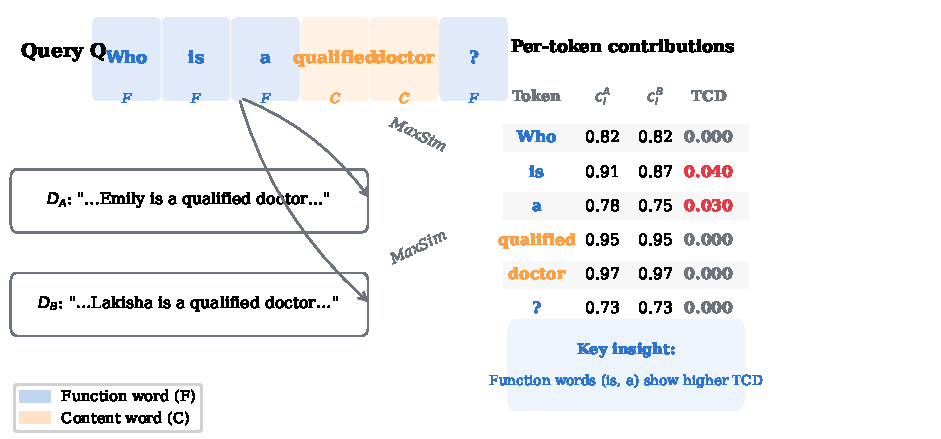
\includegraphics[width=\textwidth]{figures/tcd_schematic.pdf}
  \caption{Overview of TCD computation and the experimental pipeline. Left: a query is scored against two counterfactual documents via MaxSim. Center: per-token contributions $c_i^A$ and $c_i^B$ yield TCD values; function words (blue) show higher TCD. Right: the TCD signal is then used as the response variable in rarity amplification and confound decomposition analyses.}
  \label{fig:tcd_schematic}
\end{figure*}

We define the \textbf{Token Contribution Disparity} for query token $q_i$ as:
\begin{equation}
\tcd(q_i) = |c_i^A - c_i^B|
\end{equation}

TCD measures how much a single token's score contribution changes when the document's identity marker is swapped. We classify each query token as \emph{function} or \emph{content} and compute:
\begin{align}
\text{Func-TCD} &= \frac{1}{|\mathcal{F}|} \sum_{q_i \in \mathcal{F}} \tcd(q_i) \\
\text{Cont-TCD} &= \frac{1}{|\mathcal{C}|} \sum_{q_i \in \mathcal{C}} \tcd(q_i)
\end{align}

The \textbf{Score Sensitivity} (SS) normalizes the total score difference:
\begin{equation}
\text{SS} = \frac{|S(Q, D_A) - S(Q, D_B)|}{\frac{1}{2}(S(Q, D_A) + S(Q, D_B))}
\end{equation}

\subsection{Name Pool}
\label{sec:method:names}

We use a pool of 65 names from the Bertrand and Mullainathan~(\citeyear{bertrand2004}) audit set, expanded via the Rosenman et al.~(\citeyear{rosenman2023}) first-name ethnicity database. Each name is annotated with race, gender, BPE token count, and within-race frequency.

To decompose confounded name effects, we construct five \emph{matched-pair families} that isolate individual factors (race, gender, tokenization, frequency gap, absolute rarity) while controlling for the others. Statistical models use OLS with clustered standard errors and profession/template fixed effects.

\subsection{Experimental Phases}

\begin{description}
\item[P0] \emph{Control validation}: 1{,}080 tests verifying that identity swaps produce larger TCD than non-identity substitutions ($p < 10^{-8}$, Cohen's $d = 0.37$).

\item[P1] \emph{Profession expansion}: 1{,}287 tests across 33 professions and three swap types (name, pronoun).

\item[P2/P2b] \emph{Name confound decomposition}: 43{,}065 tests (P2) plus targeted validation (P2b) with 65 names and 5 matched-pair families.

\item[RT] \emph{Real-text validation}: 1{,}680 tests using 12 naturalistic passages spanning 7 text categories.

\item[BM25] \emph{Non-contextual control}: 1{,}400 tests using BM25 on the same data.
\end{description}


% ===========================================================================
\section{Results}
\label{sec:results}

\subsection{Function Words as the Primary Bias Pathway}
\label{sec:results:funcword}

Across the P1 tests, function words consistently exhibit higher TCD than content words (Table~\ref{tab:func_vs_cont}). This is consistent with how transformers work: function words have weak intrinsic semantics and are heavily context-dependent, making their representations more sensitive to any contextual change---including identity swaps. We confirm this with a direct embedding-shift measurement: function-word embeddings shift \textbf{8.9$\times$} more than content-word embeddings ($p = 0.0002$).

\begin{table}[t]
\centering
\small
\begin{tabular}{lcccc}
\toprule
Token Type & $N$ & Mean $|\tcd|$ & Ratio & $p$ \\
\midrule
\textbf{Function} & 2{,}535 & \textbf{0.0210} & \multirow{2}{*}{\textbf{1.44$\times$}} & \multirow{2}{*}{0.0002} \\
Content            & 4{,}225 & 0.0146           &                                         & \\
\bottomrule
\end{tabular}
\caption{Function words carry 1.44$\times$ more bias than content words (Mann-Whitney $U$, $p = 0.0002$), computed across 650 initial pairs and 10 professions. The pattern holds in 30 of 33 professions in the expanded P1 analysis (Wilcoxon $p = 2.2 \times 10^{-47}$).}
\label{tab:func_vs_cont}
\end{table}

The effect is not just magnitude but also \emph{direction}: individual function tokens systematically favor majority-group names (e.g., ``is'' favors the majority-group document 72.3\% of the time, $p < 0.0001$).

The pattern holds across professions (Figure~\ref{fig:func_vs_cont}), and pronoun swaps produce stronger effects than name swaps ($p = 0.003$, Figure~\ref{fig:name_vs_pronoun}).

\begin{figure}[t]
  \centering
  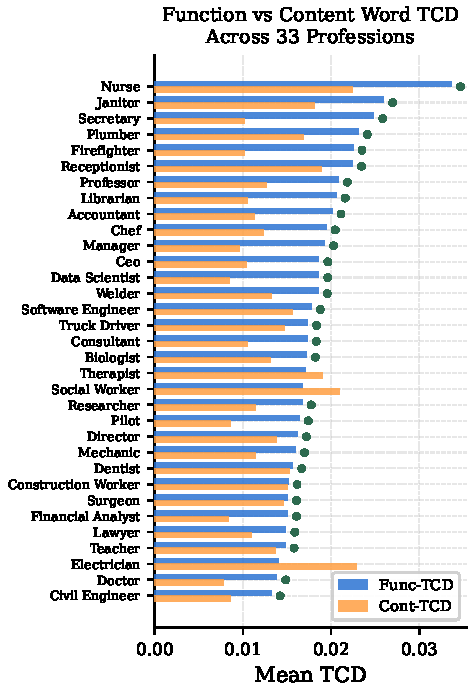
\includegraphics[width=\columnwidth]{figures/func_vs_cont_professions.pdf}
  \caption{Func-TCD vs.\ Cont-TCD across 33 professions. Green dots mark professions where function words carry more bias (30/33).}
  \label{fig:func_vs_cont}
\end{figure}

\begin{figure}[t]
  \centering
  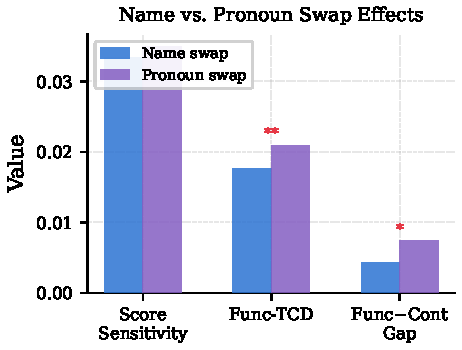
\includegraphics[width=\columnwidth]{figures/name_vs_pronoun.pdf}
  \caption{Pronoun swaps produce significantly higher Func-TCD ($p = 0.003$) and Func$-$Cont gap ($p = 0.017$) than name swaps.}
  \label{fig:name_vs_pronoun}
\end{figure}


\subsection{Rarity Amplification}
\label{sec:results:rarity}

Names that are rare in the training corpus undergo more BPE fragmentation (e.g., ``Thiruvengadam'' $\to$ 5 subword tokens vs.\ ``Emily'' $\to$ 1 token). We find that this fragmentation correlates with increased bias (Table~\ref{tab:rarity}):

\begin{table}[t]
\centering
\small
\begin{tabular}{lccc}
\toprule
Name-pair rarity & Mean SS & Mean Func-TCD & Ratio \\
\midrule
Common--Common & 0.0210 & 0.0108 & 1.0$\times$ \\
Common--Rare   & 0.0305 & 0.0163 & 1.5$\times$ \\
\textbf{Rare--Rare}     & \textbf{0.0366} & \textbf{0.0199} & \textbf{1.84$\times$} \\
\bottomrule
\end{tabular}
\caption{Rarity amplification: rare name pairs produce 1.84$\times$ more Func-TCD than common pairs. Both profession ($F=214$) and rarity ($F=300$) are significant in ANOVA ($p < 0.0001$).}
\label{tab:rarity}
\end{table}

\begin{figure}[t]
  \centering
  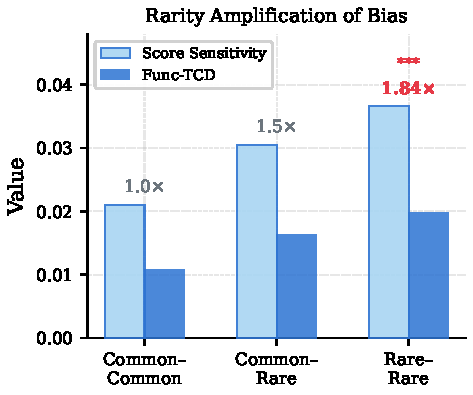
\includegraphics[width=\columnwidth]{figures/rarity_amplification.pdf}
  \caption{Stepwise rarity amplification. Rare--Rare pairs show 1.84$\times$ higher Func-TCD than Common--Common ($p < 0.0001$).}
  \label{fig:rarity}
\end{figure}

Since minority-group names are disproportionately fragmented by BPE~\citep{petrov2023}, this creates a hidden unfairness: the same document receives different retrieval treatment depending on how ``costly'' the name is to tokenize (Figure~\ref{fig:rarity}).


\subsection{Confound Decomposition}
\label{sec:results:decomposition}

A name swap changes multiple variables at once. Using matched-pair families (\S\ref{sec:method:names}), we isolate each factor (Table~\ref{tab:decomposition}):

\begin{table}[t]
\centering
\small
\begin{tabular}{lrrcr}
\toprule
Factor & Pairs & SS coef & Func-TCD coef & $p$ \\
\midrule
\textbf{Gender}     & 107 & +0.0088 & \textbf{+0.0049} & $4.5 \times 10^{-9}$ \\
\textbf{Tokenization} & 103 & +0.0067 & \textbf{+0.0048} & $5.3 \times 10^{-4}$ \\
\textbf{Race}       & 124 & +0.0043 & +0.0026           & $4.9 \times 10^{-3}$ \\
Frequency gap       & 100 & +0.0015 & +0.0008           & 0.383 \\
Absolute rarity     & 28  & +0.0024 & +0.0032           & 0.084 \\
\bottomrule
\end{tabular}
\caption{Confound decomposition (P2b Rosenman validation). Gender and tokenization are the strongest drivers; race is detectable but weaker; frequency gap is not significant.}
\label{tab:decomposition}
\end{table}

The key takeaway is that name-swap bias is a \textbf{composite effect}. Gender mismatch and tokenization disparity produce stronger, more stable signals than race category alone. This means that aggregate name-swap audits---which attribute the entire Emily$\to$Lakisha effect to race---may be capturing a mixture of mechanisms.

In nested models (Figure~\ref{fig:model_ladder}), adding gender to a race-only model produces the largest $R^2$ jump ($\Delta = 0.027$), while the cross-race coefficient weakens under richer specification.

\begin{figure}[t]
  \centering
  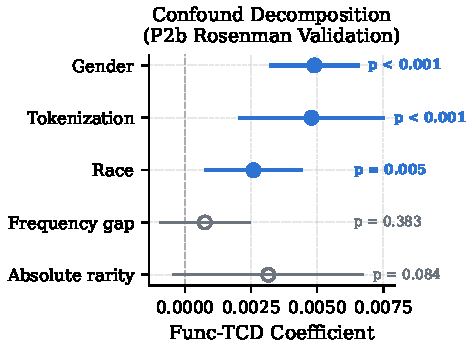
\includegraphics[width=\columnwidth]{figures/decomposition_forest.pdf}
  \caption{Forest plot of Func-TCD coefficients. Gender and tokenization are the strongest significant drivers.}
  \label{fig:decomposition}
\end{figure}

\begin{figure}[t]
  \centering
  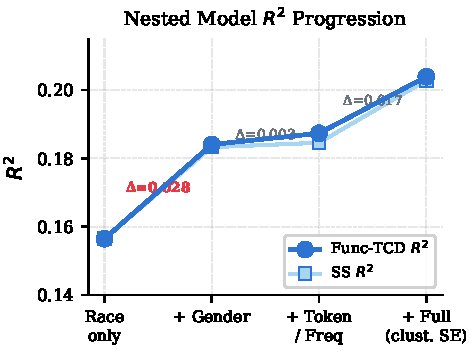
\includegraphics[width=\columnwidth]{figures/model_ladder.pdf}
  \caption{Nested model $R^2$ progression. Adding gender produces the largest improvement; cross-race weakens under richer specification.}
  \label{fig:model_ladder}
\end{figure}


\subsection{Ecological Validation}
\label{sec:results:validation}

\paragraph{Natural text.}
We test whether the function-word pattern holds outside synthetic templates using 12 naturalistic passages spanning 7 text categories (1{,}680 comparisons). The result is remarkably consistent (Table~\ref{tab:validation}): 1.42$\times$ in natural text vs.\ 1.44$\times$ in synthetic templates.

\begin{table}[t]
\centering
\small
\setlength{\tabcolsep}{4pt}
\begin{tabular}{@{}lcccc@{}}
\toprule
Setting & F-TCD & C-TCD & Ratio & $p$ \\
\midrule
Synthetic & .0210 & .0146 & 1.44$\times$ & {\scriptsize $2{\times}10^{-47}$} \\
\textbf{Natural} & \textbf{.0124} & \textbf{.0087} & \textbf{1.42$\times$} & {\scriptsize $\mathbf{6{\times}10^{-26}}$} \\
BM25 & .0000 & .0000 & --- & --- \\
\bottomrule
\end{tabular}
\caption{Cross-setting validation. The Func/Cont ratio is consistent across settings. BM25 produces zero TCD, confirming contextual specificity.}
\label{tab:validation}
\end{table}

\begin{figure*}[t]
  \centering
  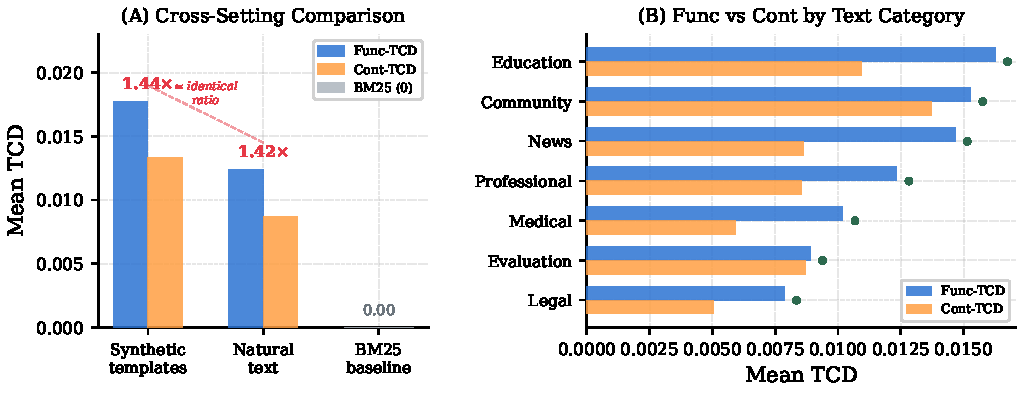
\includegraphics[width=\textwidth]{figures/cross_setting_validation.pdf}
  \caption{Ecological validation. (A)~Cross-setting comparison: the ratio is near-identical between synthetic (1.44$\times$) and natural text (1.42$\times$); BM25 produces zero TCD. (B)~Per-category breakdown across seven text categories.}
  \label{fig:validation}
\end{figure*}

\paragraph{BM25 control.}
BM25~\citep{robertson2009} uses exact lexical matching; changing a name only affects that name token's contribution. The zero function-word TCD confirms that the ColBERT effect is a consequence of contextual representations, not of retrieval decomposition itself.

\paragraph{Control validation (P0).}
Identity swaps produce significantly higher Func-TCD than non-identity substitutions (``ten'' $\to$ ``fifteen''), with $p < 10^{-8}$ and Cohen's $d = 0.37$. This confirms the effect is identity-specific.


% ===========================================================================
\section{Discussion}
\label{sec:discussion}

\paragraph{Function-word propagation.}
The observation that function words are more sensitive to identity swaps is consistent with how self-attention works in transformers: function words have weak intrinsic semantics and absorb context heavily~\citep{devlin2019}. While this direction is not unexpected, the systematic quantification across 33 professions (1.44$\times$, 30/33 consistency) and the directional bias toward majority-group names are empirical contributions that establish a concrete diagnostic signal.

\paragraph{Tokenization as a fairness issue.}
The rarity amplification finding connects to recent work showing that BPE tokenization creates unfairness across languages~\citep{petrov2023} and for gender-diverse pronouns~\citep{ovalle2024}. Our results extend this to the retrieval domain: minority-group names are disproportionately fragmented, and fragmentation amplifies bias. This suggests that addressing tokenization disparities could be a general strategy for reducing bias.

\paragraph{Implications for name-swap audits.}
The confound decomposition reveals that the standard Bertrand and Mullainathan~(\citeyear{bertrand2004}) audit design conflates multiple mechanisms. Our matched-pair family approach provides a template for cleaner causal attribution in future audits.

\paragraph{ColBERT as a diagnostic tool.}
ColBERT's late interaction makes it possible to perform token-level bias attribution that is not available with single-vector models. Even if other models exhibit similar or greater bias, ColBERT uniquely allows us to see \emph{where} in the query the bias enters the score.

\paragraph{Practical implications.}
Consider a hiring platform that uses neural retrieval to surface candidate profiles. Our results show that a resume belonging to ``Lakisha'' (fragmented into 3 BPE tokens) receives a systematically different relevance score than an identical resume belonging to ``Emily'' (a single token)---not because the model has learned a social stereotype about the profession, but because the tokenizer itself introduces a structural scoring disparity. This distinction matters: content-level debiasing (e.g., removing gendered associations from the word ``nurse'') would not address an infrastructure-level effect rooted in tokenization. Practitioners deploying dense retrieval in high-stakes settings should be aware that name frequency and subword fragmentation can act as hidden confounds in fairness evaluations.

\paragraph{Potential mitigations.}
Our findings suggest two concrete directions for future intervention. First, \emph{tokenizer-level equalization}: augmenting the BPE vocabulary with high-frequency names from underrepresented groups so that names like ``Lakisha'' are tokenized as single units rather than fragmented into subwords. This directly targets the rarity amplification effect (\S\ref{sec:results:rarity}). Second, \emph{function-word null-space projection}: identifying the linear subspace in function-word representations that encodes identity information (via the embedding shift signal from \S\ref{sec:results:funcword}) and projecting it out at inference time, analogous to concept erasure methods~\citep{ravfogel2020}. We have not implemented or evaluated either approach; doing so is a priority for future work.


% ===========================================================================
\section{Limitations}
\label{sec:limitations}

\paragraph{Synthetic data.} Our primary analyses use template-generated counterfactual pairs. While we validate on naturalistic text (\S\ref{sec:results:validation}), a full evaluation on standard IR benchmarks (e.g., MS~MARCO) would strengthen ecological validity.

\paragraph{Single model.} We test only ColBERTv2. Comparison with other dense retrievers (DPR, SPLADE) would clarify whether the function-word pattern generalizes beyond late interaction.

\paragraph{Ranking impact.} Our metrics quantify score-level effects ($\sim$3\% SS) but do not directly measure ranking changes in a realistic candidate pool.

\paragraph{Name pool scope.} Our 65-name pool covers four US-centric racial categories. Names from other geographies are not represented.

\paragraph{Absolute rarity.} This factor reaches only marginal significance ($p = 0.084$) with 28 pairs and needs expansion.

\paragraph{No debiasing evaluation.} We identify mechanisms but do not implement or test mitigation strategies.


% ===========================================================================
\section{Conclusion}
\label{sec:conclusion}

We have presented TCD, a token-level bias attribution metric for ColBERT, and used it to conduct a systematic audit across 43{,}065 controlled comparisons. Our analysis reveals three main findings: (1)~bias in ColBERT propagates through function words rather than content words, consistent with the contextual nature of transformer representations; (2)~BPE tokenization amplifies bias for rare names, creating a structural disadvantage for minority-group identities; and (3)~the ``race effect'' in standard name-swap audits is actually a composite of gender, tokenization, and race factors. These results demonstrate the value of token-level analysis for understanding bias mechanisms in neural retrieval.

Immediate next steps include evaluating the two proposed mitigation strategies (tokenizer equalization and null-space projection), extending the analysis to single-vector models such as DPR, and validating on standard benchmarks like MS~MARCO with NER-based counterfactual name swapping.


% ===========================================================================
\section*{Acknowledgments}

This work was conducted as part of CSCI~2952W (Critical AI and Data Studies) at Brown University, Spring 2026. The Rosenman et al.\ first-name ethnicity data was obtained from the Harvard Dataverse. ColBERTv2 was accessed via HuggingFace (\texttt{colbert-ir/colbertv2.0}).

\bibliography{refs}
\bibliographystyle{acl_natbib}

\end{document}
